\documentclass[../root]{subfiles}
\graphicspath{{_images/}{../_images/}}

\begin{document}

    \chapter{Cognitive Mobility: Labor Market Responses to Supply Shocks in the Space of Ideas}

    \begin{shortsummary}
        \begin{itemize}
            \item \authoryear{Kato2013} 
            \item \RQ{Does the decreasing of H1-B visa affect student score ?}
            \item \answer{This paper use Difference-in-difference method and some robustness check.}
            \item \result{The restriction of high skilled immigrants cause decreasing the student score.}
        \end{itemize}
    \end{shortsummary}

    \section{Introduction}
   Foreign students often study in the United. States in hoping that an American undergraduate education will serve as a gateway to long-term U.S. employment.
   
   \begin{itemize}
       \item  Bhagwati and Rao (1999) andChiswick (1999) claim that student that student visa are often used in hopes of securing permanent employment.
       \item It follow that a foreign student considering higher education in U.S will be affected by any exogenous change.
       \item In October 2003, the U.S. limited the new H-1B visa issuance per annum dramatically fell from 195,000 to 65,000. 
   \end{itemize}
   The H-1B visa was never binding in the year immediately preceding the policy change.
   Thus, Foreign citizens with undergraduate degrees faced no legal impediment to working in the U.S. as they had received a job offer from an employer. 
   
   The U.S. visa quotas in general reduce the U.S. immigrant inflows is already well established in the literature.
   
   {\bf Research Question and how to answer it}
   \begin{itemize}
       \item  This paper assesses how restriction H-1B policy has affected the average academic quality of prospective international students who face reduced U.S. employment opportunity after graduation. 
       \item For some countries, the U.S. provided alter visas and these countries were affected little effect by H1-B policy change. This paper use Difference-in-difference method to estimate the causal effect.
   \end{itemize}
  
   From DID estimation, this paper show that H-1B policy reduce the student SAt score. This results are robust in some robust check. 
   
   
    \section{Literature and Motivation}
    
    Economist have highlight the potential for both positive and negative effect of highly educated immigrants.
    
    \begin{itemize}
        \item The negative effect means that highly educated immigrants could reduce native employment and wage opportunity.
        \item The positive effect means that the highly educated immigrants could cause innovation and entrepreneurial.
    \end{itemize}
     
     Less work has been done on the effect policy on the quality of immigrants.
     For research on skilled immigrants quality issue may be even more important than quantity.
     
     \begin{itemize}
         \item  Rosenzweig (2006) focus on the determinants of foreign student flow because student flows are considerably larger than other skill-based flows, while there is no country-specific or total ceiling on student visas.
            \begin{itemize}
                \item He reports students are likely to be motivated by economics.
                \item He conclude foreign student go to the United States in hopes of permanent employment.
            \end{itemize}
         \item Chiswick (2000) argues that migrants are favorably self-selection. If the direct costs of migration rise or if ability is negative correlative with the costs of migration, this favorable self-selectivity grows strongly. 
         \item  Chen (2005) provides that the quality of masters degree students in a Chinese university and their interest in migration to the the United States for continued education.  
         \begin{itemize}
             \item He finds that potential emigrations were negatively self-selected during a less restricted during a less restrictive policy regime but positively self-restricted during a more restricted regime.
         \end{itemize}
     \end{itemize}
     
     This paper aim to show the relationship between the restrictive H-1B policy change and the quality of immigrants.
     
     \section{Empirical Strategy}
    
    
    
    {\bf Empirical hypothesis}
    
    \begin{itemize}
        \item If high-ability students are particularly sensitive to labor policy change, immigration restriction could reduce the average quality of international application to U.S. high education.
        \item The opposite prediction is also theoretically possible. If low-ability think they could not take H-1B visa, low-ability students more sensitive to restrict policy. Thus, average quality of foreign-students increase.   
    \end{itemize}
    
    {\bf History of H-1B policy}
    
    The immigration Act of 1990 created H-1B visa for professional foreign national seeking employment in the United States.
    
    Figure 1 represents 1\% rise in undergraduate enrollment is associate with an equivalent rise in H-1B visa issued four year later, controlling for country population size.
    
    \begin{figure}
        \centering
        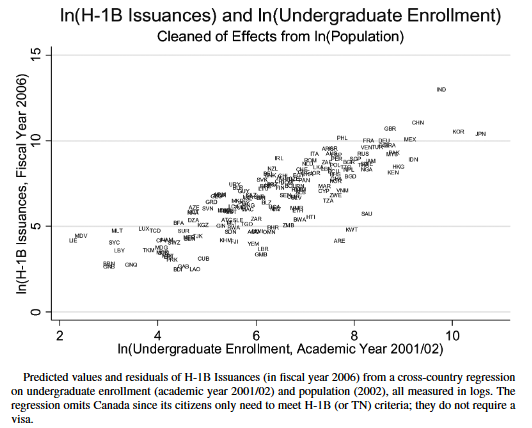
\includegraphics[width = \linewidth]{1016sugiyama/Figure_1.png}
        \caption{Figure.1 H-1B Issuances and Undergraduate Enrollment}
        \label{fig:my_label}
    \end{figure}
    
    At the time to its creation, 65,000 H-1B visas became available for new application each year.
    
    Cognitive responded to the the increase in demand for H-1B visa with the American Competitiveness in the 21st Century Act (AC21). 
    
    In authors' research design, potential foreign applicants to U.S. colleges can be seen as having received a "treatment" in fall 2003. 
    
    Potential foreign applicants from five key countries were unaffected by this treatment and H-1B visa cap reduction, Canada, Mexico, Chile, Singapore, and Australia.
    
    Free treatment agreement have created close H-1B substitution for citizens from these countries.
    
    Figure 2 demonstrates that workers from these countries indeed choose alternative route of entry.
    
    \begin{figure}
        \centering
        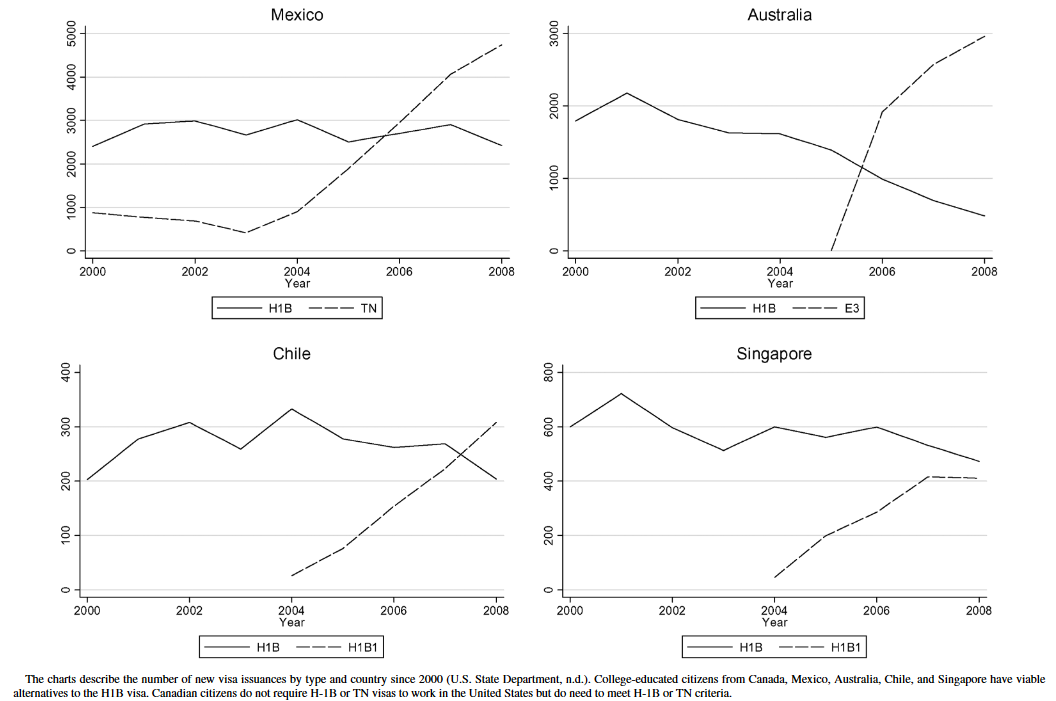
\includegraphics[width = \linewidth]{1016sugiyama/Figure_2.png}
        \caption{Figure 2. Visa Issuances}
        \label{fig:my_label}
    \end{figure}
    
    In term of research design, foreign applicants from these countries from a control group, and all of other foreign applicants comprise a treatment group.
    
    Evidence that restrictive H-1B policy reduced the number of foreign undergraduates instead in U.S. education can be seen from the Institution of  International Education (IIE).
   
   {\bf Student Ability Data}
   
   The authors use STA score as a measure of applicant ability.
   
   Rask and Tiefenthaler (2009, p. 1) note that "the chief complaint against the SAT is that it is not the best predictor of college success but is highly correlated with parental education and income".
   
   Most SAT critiques focus on its ability to predict domestic student success.
   
   \begin{itemize}
       \item The primary data source is the College Board, which owns the SAT.
       \item School type and their characteristics are determined by the $2009 \ US \ News \ and \ World \ \\
       Report \ Guide \ to \ American's \ Best \ College \ (USNWR)$. USNWR provides a single rank of U.S. college and unversity.
   \end{itemize}
   
   They use this ranking to create labeling of college and university.
   \begin{itemize}
       \item They label research and liberal arts school in the top 50 as "top tier"
       \item 51 to 100 and other tier 1 as "middle tier"
       \item tier 3 and tier 4 are "bottom tier".
   \end{itemize}
   
   \begin{figure}
        \centering
        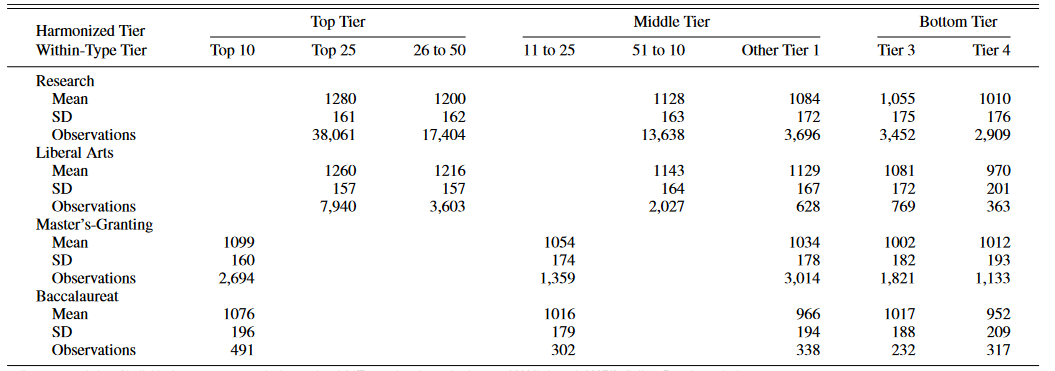
\includegraphics[width = \linewidth]{1016sugiyama/Table_1.png}
        \caption{Table.1 Average SAT Scores of Potential International Applicants by Type and Tier of School}
        \label{fig:my_label}
    \end{figure}
   
   The observation is 106,191.
   
   {\bf Main Regression Specification}
   
   To identify the effect of H-1B visa policy on the ability of prospective applicants from abroad, they estimate the difference-in-difference model in equation (1):
   \begin{align}
       Scores_{x,c,t} = \alpha + \beta \cdot H1B_{s,c,t} +\delta_s + \delta_c+\delta_t + \epsilon_{s,c,t}
   \end{align}
   
   The variable of $Score$ is the measure of academic quality of international applicants, measured by the average math, verbal, or combined SAT score reports received pseudo-school $s$ who from students who last took the exam in country $x$ at date $t$.
   
   The  main coefficient of interest, $\beta$ , measures the effect of restrictive H-1B visa policy on the quality of score received by schools from foreign students interested in U.S. education.
   
   The variable $H1B$ equal to 0 for individuals taking the exam on or before 2003; those from Canada, Chile, Mexico, and Singapore in any year; and those from Australia at all dates expect November 2003 through May 2005. The variable equals to 1 for all other observations.  
   
   This implies that $\beta$ will be negative if current visa policy has caused U.S.
   
   Two concern to the validity of their difference-in-difference methodology.
   
   \begin{enumerate}
       \item The exogeneity of policy variable. This is seem unlikely. 
       \begin{itemize}
            \item H1-B visa regime was likely motivated by macroeconomic forces that apply to interest immigrants from all countries.
            \item Variation in policy across countries is unrelated to macroeconomic condition.
         \end{itemize}
         \item Identification would arise treatment and five countries had experienced differential trends in SAT performance prior to the change in H-1B policy 
         \begin{itemize}
            \item Between academic years 2000/1 and 2002/3, average SAT scores rose 4\$ for treatment countries that would later H-1B restrictive.
            \item Scores rose a qualitatively equal 39\% for control countries.
            \item Prepolicy regression reveal no relationship between the trend in scores received by pseudo-school and whether scores are coming from treatment and control countries. 
         \end{itemize}
   \end{enumerate}
   \section{Results}
   
   {\bf Main Results from College Board Data}
   
   Baseline results are in the table 3.
   
   \begin{figure}
        \centering
        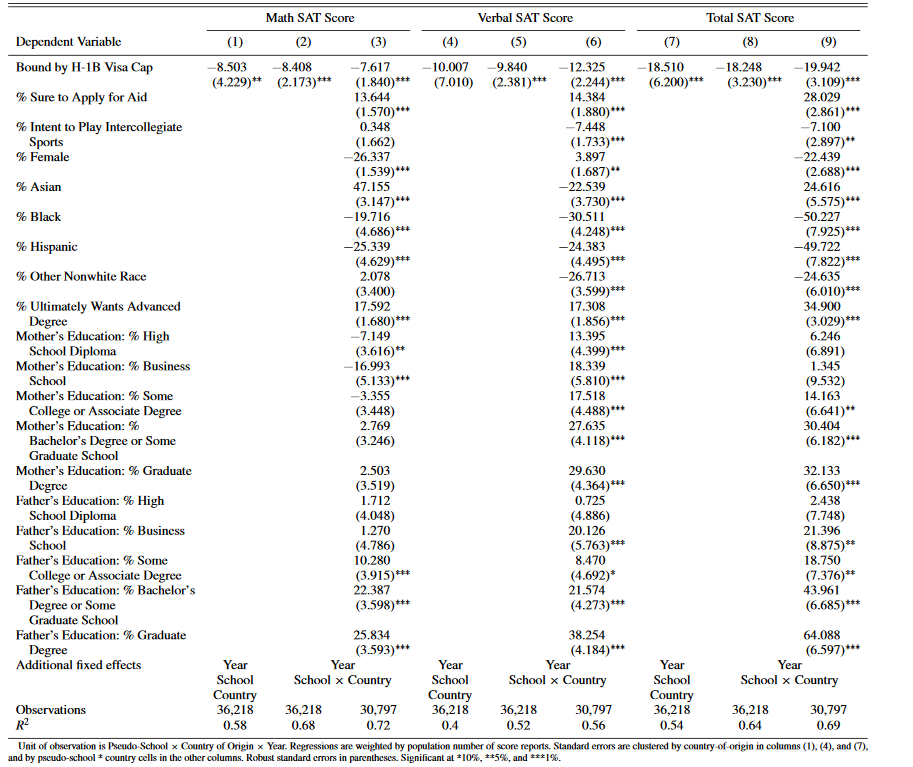
\includegraphics[width = \linewidth]{1016sugiyama/Table_3.png}
        \caption{Table.3 Baseline Results, College Board Data}
        \label{fig:my_label}
    \end{figure}
   
   \begin{itemize}
       \item The first specification for each dependent variable  includes origin country plus receiving school fixed effect.
       \item Standard errors are clustered by country.
       \item The second and third instead use School $\times$ Country fixed effect with standard errors clustered by this unique identifier. 
   \end{itemize}
   
   The estimated coefficients on $H1B_{s,c,t}$ when applicant characteristic are not controlled for are negative and statistically significant at least at the 5\% level expect when the average SAT verbal score is used as the dependent variable. 
   
   {\bf Timing Issues in Identifying Average Score Effect}
   
   The authors explore potential seasonality in the data. Since their data set dose not identify the number of times an individual has taken the exam, but they can account for seasonality by controlling for the month and year in which an exam was taken.
   
   \begin{itemize}
       \item The first row of results n column 1 to 3 of table 5 represents the regressions in column 2, 5, 8 of table 3, but they replace year indicators with year-by-month exam date fixed effects.
       \item One limitation of this approach is that the SAT is not offered in all countries on all potential exam dates.
   \end{itemize}
   
   The results with controlling month variable show that more large reduction. This tendency is shown in the math score.
   
   
   They assume that the foreign student response soon as the policy change. This is checked by column 4 and 5 of table 5. From this results, the assumption should be valid.
   
   They also check if the College Board data set does not measure on which a student elects to send a score report to a given school.
   
   \begin{itemize}
       \item This is problem if student who had taken the exam before the policy change then respond to it by selecting a new group of school to receive reports.
       \item Column 6 addresses this issue by assuming that people apply to matriculate to universities in the fall of the year following their SAT date.
       \item Column 6 indicates that the SAT quality response to H-1B policy is robust to timing assumption. 
   \end{itemize}
   
   \begin{figure}
        \centering
        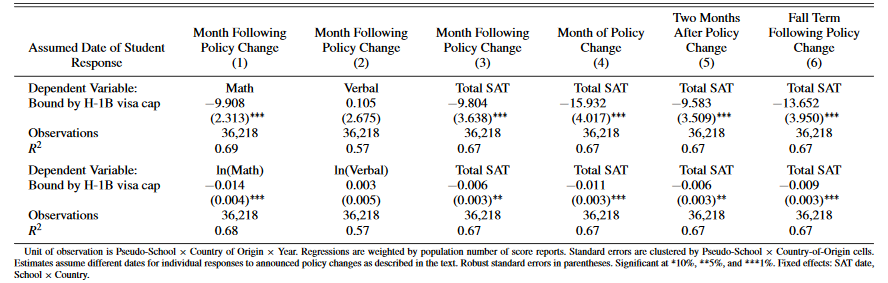
\includegraphics[width = \linewidth]{1016sugiyama/Table_5.png}
        \caption{Table.5 Timing of Policy and SAT Score Response, Varied Approaches}
        \label{fig:my_label}
    \end{figure}
    
    \begin{figure}
        \centering
        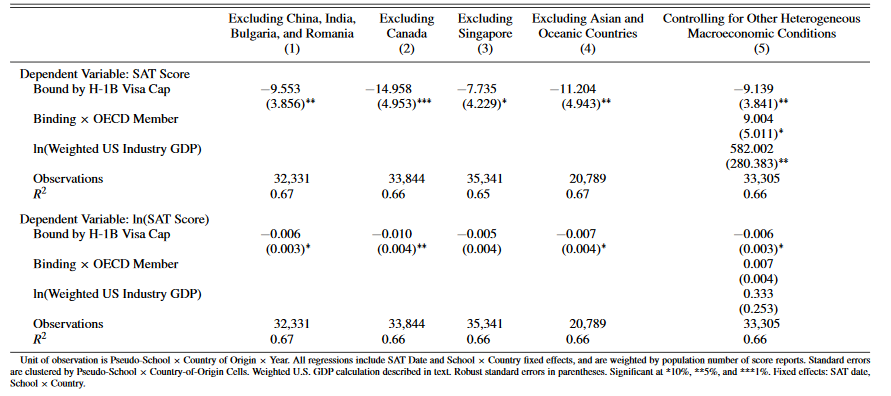
\includegraphics[width = \linewidth]{1016sugiyama/Table_6.png}
        \caption{Table.6 Controlling for Macroeconomic Conditions}
        \label{fig:my_label}
    \end{figure}
    
    
   {\bf Macroeconomic Condition and Country Exclusion}
   
   Estimation of equation (1) could be biased if U.S. policy dates are correlated with country-specific macroeconomic events or trend.
   
   In table 6, the empirical specification is comparable to column 3 of table 5.
   
   \begin{itemize}
       \item Column 1 considers countries bound by H-1B constrains that experienced unique changes during their period of analysis.
       \begin{itemize}
           \item China and India are undergoing rapid economic development.
           \item Bulgaria and Romania signed the Treaty of Accession to European Union in April 2005.
           
       \end{itemize}
       \item Roughly two-third of scores reports among control countries come from Canadian, and another quarter come from Singapore. Column 2 and 3 omit score reports sent from citizens of these respective countries.
       \item Countries near the South Korea and Australia that could serve primary south of their foreign student body. So in column 4, they omit Asian and Oceanic countries.
   \end{itemize}
   
   In column 5, they control for heterogeneous macroeconomic condition. There are two reason to control for macro economic condition.
   
   \begin{enumerate}
       \item Prospective students from less developing countries have stronger incentive to work permanently in America and more sensitive to -1B policy.
       \item Trough year fixed effect account for macroeconomic conditions, those conditions might have a heterogeneous effect if economic fluctuations and country-specific immigrant representation vary across industry.  
   \end{enumerate}
   
   To control this heterogeneity, they use follow variable.
   \begin{itemize}
       \item They use BEA data on U.S. industrial output (GDP) produced in nineteen sector in each year ($GDP_{i,t}$, where $i$ = industry, t =  year).
       \item They also use census data from King et al.(2000) to calculate the fraction of origin country's college-educated U.S. migration workforce employment in each industry in 2000 ($L_{c, i, 2000}/L_{c, 2000}$).  
       \item From these data, they compute the weighted average of industry-level U.S. GDP relevant to a college-educated potential U.S. immigrant worker from country $c$ in year $t$:
       \begin{align}
           Weighted \ Industry \ GDP_{c, t} = \sum^{19}_{i=1} GDP_{i, t} \cdot \left(\frac{L_{c, i, 2000}}{L_{c, 2000}} \right) 
       \end{align}
   \end{itemize}
   
   The result of column 5 is robust to the column 3 of table 5.  
   
   Column 5 suggest some tendency.
   \begin{itemize}
       \item OECD interaction term is significant and positive. SAT scores from developed countries are indeed less affected by restricted H-1B policy than developing countries are.
   \end{itemize}
   
   {\bf Compositional and Demographic Effects}
   
   Table 7 checks whether the effects differ across type and quality of institution. 
   \begin{itemize}
       \item Column 1 shows the different effect of each field.
       \item Column 2 shows the different effect of school ranking.
   \end{itemize}
   
   \begin{figure}
        \centering
        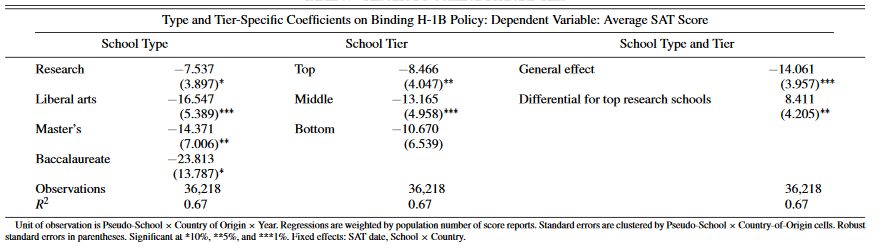
\includegraphics[width = \linewidth]{1016sugiyama/Table_7.png}
        \caption{Table.7 Results by College Type and Tier}
        \label{fig:my_label}
    \end{figure}
   
   Table 8 shows that the policy's effect on the demographic composition of potential applicants.
   
   \begin{figure}
        \centering
        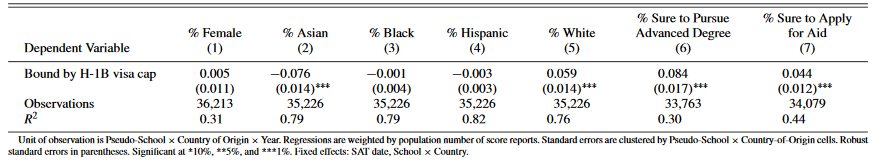
\includegraphics[width = \linewidth]{1016sugiyama/Table_8.png}
        \caption{Table.8 Effect of Restrictive H-1B Policy on Demographic Composition of Prospective International Students}
        \label{fig:my_label}
    \end{figure}
    
    \begin{itemize}
        \item Asian students decrease by 7.6 percentage points, wile white students increase by 5.9 percentage points. 
        \item Column 6 shows that H-1B policy has increased the proportion of a applicants intending to continue their education after obtaining a bachelor's degree. 
        \item Column 7 suggests that the policy change has caused demand for financial students to increase. The reason why the internal students have lower expected benefit from U.S. education.
    \end{itemize}
    
    {\bf Quintile Regression}
    College and policy maker might have a particular interest in whether the observed drop in average ability comes mostly from reduced interest among high-ability students or a rise in applicants from low-ability students.  
    
    
    The authors calculate the share $r$ of a pseudo-school's report ($R$) from country $x$ at time $t$ belong to each quintile $q$, that is $r_{s,c,t,q} = \frac{R_{s,c,t,q}}{R_{s,c,t}}$, where $R_{s,c,t} = \sum^5_{q=1} R_{s,c,t,q}$.
    
    \begin{figure}
        \centering
        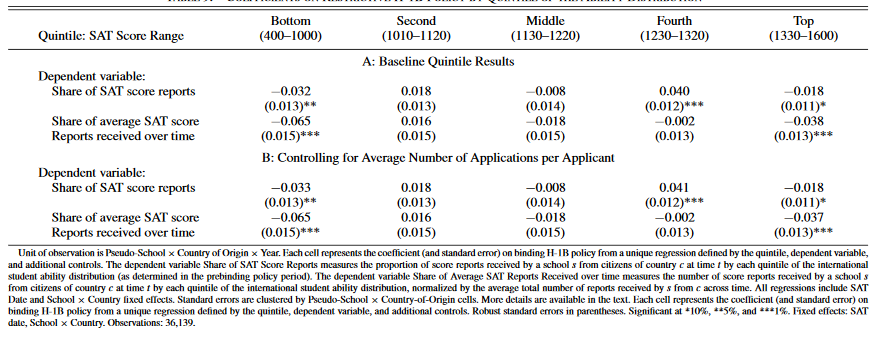
\includegraphics[width = \linewidth]{1016sugiyama/Table_9.png}
        \caption{Table.9 Coefficients on Restrictive H-1B Policy by Quintile of the Ability Distribution}
        \label{fig:my_label}
    \end{figure}
    
    From the results, the restrictive policy reduces the share of bottom and top students, and increases the share of fourth students. This tendency is stronger in the regression controlling average number of applicants. 
    
    {\bf Case study}
    
    The College Board data present three problems.
    \begin{itemize}
        \item It data set provides only one measure, SAT score, some researchers consider an inferior measure of applicant ability at compared to high school GPA.
        \item The College Board data cannot be strictly interpreted as a applicants but is rather a sample of foreign prospective applicants. We cannot distinguish between the applicants and those who sent SAT scores to U.S. schools but later declined to submit a formal.  
        \item Results may counfounded by remaining timing issue, including the challenge of precisely identifying the dates on which individual behaviour would respond to a policy change.
    \end{itemize}
    
    They use second data set to account to these problems.
    
    \begin{itemize}
        \item It includes every foreign national officially applying to matriculate at a particular highly selective university between fall 2001 and fall 2008.
        \item The authors drop individuals who have dual U.S. citizenship or are permanent U.S.  residual.
        \item The use of applicants data reduces ambiguity surrounding the timing of applicants.  Students should aware of the current policy at the time of application submission.
        \item The data set contains high school GPA.
    \end{itemize}
    The dependent variable reflect the average abilities of applicants to this particular university.
    
    The authors assume that students perceived H-1B policy to unbinding 
    \begin{itemize}
        \item if they enter college before 2004.
        \item if they applied from Canada, Chile, Mexico, and Singapore in any year
        \item if they were from Australia applying to enter college in except 2004.
    \end{itemize}
      
      \begin{figure}
        \centering
        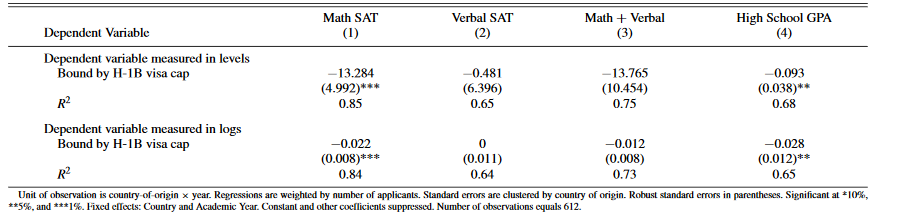
\includegraphics[width = \linewidth]{1016sugiyama/Table_10.png}
        \caption{Table.10 Case Study of Applicants to a Highly Selective University}
        \label{fig:my_label}
    \end{figure}
    
    In those results, the impact on math is negatively significant and the impact on verbal are not significant. The authors consider that this is because of sample size. 
    
    The column 4 shows that H-1B policy also reduces high school GAP same as SAT scores. This results means H-1B policy change reduces applicants ability.
    
    
    \section{Summary}
    
    This paper employs two data:
    \begin{itemize}
        \item College Board data on the SAT scores of prospective student 
        \item SAT and GPA data on a highly selective university's foreign applicants.
    \end{itemize}
    Both cases generate robust evidence that limits on H-1B immigration of educated labor have had an unintended adverse effect on U.S. higher education by reducing the average ability of potential foreign applicants.
    
    Quintile regression shows that the share of the applicants from the top-quintile students decline by 1.8 to 3.7 percentage points. 
    
    \biblio
    
\end{document}